%---------------------------------------------------------------------------%
%-                                                                         -%
%-                           LaTeX Template                                -%
%-                                                                         -%
%---------------------------------------------------------------------------%
%- Copyright (C) Huangrui Mo <huangrui.mo@gmail.com> 
%- This is free software: you can redistribute it and/or modify it
%- under the terms of the GNU General Public License as published by
%- the Free Software Foundation, either version 3 of the License, or
%- (at your option) any later version.
%---------------------------------------------------------------------------%
%->> Document class declaration
%---------------------------------------------------------------------------%
\documentclass[twoside]{Style/ucasthesis}%
%- Multiple optional arguments:
%- [<oneside|twoside|print>]% oneside eprint, twoside eprint, or paper print
%- [fontset=<adobe|none|...>]% specify font set instead of automatic detection
%- [scheme=plain]% thesis writing of international students
%- [draftversion]% show draft version information
%- [standard options for ctex book class: draft|paper size|font size|...]%
%---------------------------------------------------------------------------%
%->> Document settings
%---------------------------------------------------------------------------%

\usepackage[super,list,table,math]{Style/artratex}
%- usage: \usepackage[option1,option2,...,optionN]{artratex}
%- Multiple optional arguments:
%- [bibtex|biber]% set bibliography processor and package
%- [<numbers|super|authoryear|alpha>]% set citation and reference style
%- <numbers>: textual: Jones [1]; parenthetical: [1]
%- <super>: textual: Jones superscript [1]; parenthetical: superscript [1]
%- <authoryear>: textual: Jones (1995); parenthetical: (Jones, 1995)
%- <alpha>: textual: not available; parenthetical: [Jon95]
%- [geometry]% reconfigure page layout via geometry package
%- [lscape]% provide landscape layout environment
%- [xhf]% disable header and footer via fancyhdr package
%- [color]% provide color support via xcolor package
%- [background]% enable page background
%- [tikz]% provide complex diagrams via tikz package
%- [table]% provide complex tables via ctable package
%- [list]% provide enhanced list environments for algorithm and coding
%- [math]% enable some extra math packages
%- [xlink]% disable link colors
\usepackage{Style/artracom}% user defined commands
%---------------------------------------------------------------------------%
%->> Document inclusion
%---------------------------------------------------------------------------%
%\includeonly{Tex/Chap_1,...,Tex/Chap_N}% selected files compilation
%---------------------------------------------------------------------------%
%->> Document content
%---------------------------------------------------------------------------%
%-
%-> Titlepage information
%-

%---------------------------------------------------------------------------%
%->> Titlepage information
%---------------------------------------------------------------------------%
%-
%-> 中文封面信息
%-
\confidential{}% 密级:涉密论文或延迟公开论文填写
\schoollogo[scale=0.095]{ucas_logo}% 校徽
\title{中国科学院大学学位论文 LaTeX 模板 }% 论文中文题目
\author{论文作者}% 论文作者
\advisor{李四~教授~中国科学院xxx研究所\\}% 指导教师:姓名 专业技术职务 工作单位
%\advisor{指导教师一\\指导教师二\\指导教师三}% 多行指导教师示例
\degree{博士}% 学位:学士、硕士、博士
\degreetype{工学}% 学位类别:理学、工学、工程、医学等
\major{计算机应用技术}% 一级/二级学科专业名称,领域名称需要与学籍信息一致
\institute{中国科学院xxx研究所}% 院系名称
%\institute{中国科学院力学研究所\\流固耦合实验室}% 多行院系名称示例
\date{2023~年~6~月}% 毕业日期:夏季为6月、冬季为12月
%-
%-> 英文封面信息
%-
\TITLE{LaTeX Thesis Template of UCAS}% 论文英文题目
\AUTHOR{Author Name}% 论文作者
\ADVISOR{Supervisor: Professor LI Si}% 指导教师
\DEGREE{Doctor}% 学位:Bachelor, Master, Doctor, Postdoctor。封面据英文学位名称自动切换,需确保拼写准确
\DEGREETYPE{Philosophy}% 学位类别:Philosophy, Natural Science, Engineering, Economics, Agriculture 等
\MAJOR{Computer Application Technology}% 二级学科专业名称
\INSTITUTE{Institute of xxx, Chinese Academy of Sciences}% 院系名称
\DATE{June, 2023}% 毕业日期:夏季为June、冬季为December
%---------------------------------------------------------------------------%
%
\begin{document}
%-
%-> Frontmatter: title page, abstract, content list, symbol list, preface
%-

\frontmatter% initialize the environment
%---------------------------------------------------------------------------%
%->> Frontmatter
%---------------------------------------------------------------------------%
%-
%-> 生成封面
%-

\maketitle% 生成中文封面
\MAKETITLE% 生成英文封面
%-
%-> 作者声明
%-
\makedeclaration% 生成声明页
%-
%-> 中文摘要
%-
\intobmk\chapter*{摘\quad 要}% 显示在书签但不显示在目录
\setcounter{page}{1}% 开始页码
\pagenumbering{Roman}% 页码符号

中文摘要、英文摘要、目录、论文正文、参考文献、附录、致谢、攻读学位期间发表的学术论文与其他相关学术成果等均须由另页右页(奇数页)开始。

\keywords{中国科学院大学,学位论文,模板}% 中文关键词
%-
%-> 英文摘要
%-
\intobmk\chapter*{Abstract}% 显示在书签但不显示在目录

Chinese abstracts, English abstracts, table of contents, the main contents, references, appendix, acknowledgments, author's resume and academic papers published during the degree study and other relevant academic achievements must start with another right page (odd-numbered page).
    %- the current style, comment all the lines in plain style definition.

\KEYWORDS{University of Chinese Academy of Sciences, Thesis, LaTeX Template}% 英文关键词

\pagestyle{enfrontmatterstyle}%
\cleardoublepage\pagestyle{frontmatterstyle}%

%---------------------------------------------------------------------------%
% title page, abstract
\fancypagestyle{figureheader}{
  \fancyhf{}
  \fancyhead[C]{\footnotesize 图表目录}%此处填写中文标题
  \fancyfoot[C]{\footnotesize \thepage}% page number
    \renewcommand{\headrulewidth}{0.8pt}% header rule
    \renewcommand{\footrulewidth}{0pt}% footer rule
}
{% content list region
\linespread{1.2}% local line space
\intobmk*{\cleardoublepage}{\contentsname}% add link to bookmark
\tableofcontents% content catalog

\intobmk*{\cleardoublepage}{图表目录}
\thispagestyle{noheaderstyle}
{
\renewcommand*{\addvspace}[1]{}
\let\oldnumberline\numberline%
\renewcommand{\numberline}{\figurename~\oldnumberline}%
\listoffigures%
}
{
\let\cleardoublepage\relax
\let\clearpage\relax
\renewcommand*{\addvspace}[1]{}
\let\oldnumberline\numberline%
\renewcommand{\numberline}{\tablename~\oldnumberline}%
\listoftables%
}

\thispagestyle{figureheader}
}
\intobmk\chapter*{符号列表}% 显示在书签但不显示在目录

\section*{字符}
\nomenclatureitem[\textbf{Unit}]{\textbf{Symbol}}{\textbf{Description}}
\nomenclatureitem[$\Unit{m^{2} \cdot s^{-2} \cdot K^{-1}}$]{$R$}{the gas constant}
\nomenclatureitem[$\Unit{m^{2} \cdot s^{-2} \cdot K^{-1}}$]{$C_v$}{specific heat capacity at constant volume}
\nomenclatureitem[$\Unit{m^{2} \cdot s^{-2} \cdot K^{-1}}$]{$C_p$}{specific heat capacity at constant pressure}
\nomenclatureitem[$\Unit{m^{2} \cdot s^{-2}}$]{$E$}{specific total energy}
\nomenclatureitem[$\Unit{m^{2} \cdot s^{-2}}$]{$e$}{specific internal energy}
\nomenclatureitem[$\Unit{m^{2} \cdot s^{-2}}$]{$h_T$}{specific total enthalpy}
\nomenclatureitem[$\Unit{m^{2} \cdot s^{-2}}$]{$h$}{specific enthalpy}
\nomenclatureitem[$\Unit{kg \cdot m \cdot s^{-3} \cdot K^{-1}}$]{$k$}{thermal conductivity}
\nomenclatureitem[$\Unit{kg \cdot m^{-1} \cdot s^{-2}}$]{$S_{ij}$}{deviatoric stress tensor}
\nomenclatureitem[$\Unit{kg \cdot m^{-1} \cdot s^{-2}}$]{$\tau_{ij}$}{viscous stress tensor}
\nomenclatureitem[$\Unit{1}$]{$\delta_{ij}$}{Kronecker tensor}
\nomenclatureitem[$\Unit{1}$]{$I_{ij}$}{identity tensor}

\section*{算子}
\nomenclatureitem{\textbf{Symbol}}{\textbf{Description}}
\nomenclatureitem{$\Delta$}{difference}
\nomenclatureitem{$\nabla$}{gradient operator}
\nomenclatureitem{$\delta^{\pm}$}{upwind-biased interpolation scheme}

\section*{缩写}
\nomenclatureitem{CFD}{Computational Fluid Dynamics}
\nomenclatureitem{CFL}{Courant-Friedrichs-Lewy}
\nomenclatureitem{EOS}{Equation of State}
\nomenclatureitem{JWL}{Jones-Wilkins-Lee}
\nomenclatureitem{WENO}{Weighted Essentially Non-oscillatory}
\nomenclatureitem{ZND}{Zel'dovich-von Neumann-Doering}

% symbol list, preface content
%-
%-> Mainmatter
%-
\mainmatter% initialize the environment
\renewcommand{\labelenumi}{(\arabic{enumi}) }
\renewcommand{\labelenumii}{(\arabic{enumi}).\arabic{enumii}}
\renewcommand{\labelenumiii}{(\arabic{enumi}).\arabic{enumii}.\arabic{enumiii}}
\renewcommand{\labelenumiv}{(\arabic{enumi}).\arabic{enumii}.\arabic{enumiii}.\arabic{enumiv}}
%---------------------------------------------------------------------------%
%->> Main content
%---------------------------------------------------------------------------%
\renewcommand{\thefigure}{\thechapter-\arabic{figure}}
\renewcommand{\thetable}{\thechapter-\arabic{table}}
\renewcommand{\theequation}{\thechapter-\arabic{equation}}
\chapter{绪论}\label{chap:introduction}

\section{背景}

2022年修订的《中国科学院大学研究生学位论文撰写规范和指导意见》(以下简称《指导意见》)从2023年冬季批次开始实施。为方便各位同学使用,特提供此模板。

您在使用此模板进行学位论文撰写时,只需根据《指导意见》在相应章节填写具体内容即可。

本模板在第2章提供了本模板的使用说明,在第3章中提供了《指导意见》中关于内容和格式的部分要求,请仔细阅读。


\section{系统要求}\label{sec:system}
\begin{table}
    \bicaption{\quad 支持的LaTeX编译系统和编辑器}{\quad Supported LaTeX compiler and editor}% caption
    \footnotesize% fontsize
    \setlength{\tabcolsep}{4pt}% column separation
    \renewcommand{\arraystretch}{1.5}% row space 
    \centering
    \begin{tabular}{lcc}
        \hline
        %\multicolumn{num_of_cols_to_merge}{alignment}{contents} \\
        %\cline{i-j}% partial hline from column i to column j
        操作系统 & LaTeX编译系统 & LaTeX文本编辑器\\
        \hline
        Windows & \href{https://www.tug.org/texlive/acquire-netinstall.html}{TexLive Full} 或 \href{https://miktex.org/download}{MiKTex} & \href{http://www.xm1math.net/texmaker/}{Texmaker}\\
        Linux & \href{https://www.tug.org/texlive/acquire-netinstall.html}{TexLive Full} & \href{http://www.xm1math.net/texmaker/}{Texmaker} 或 Vim\\
        MacOS & \href{https://www.tug.org/mactex/}{MacTex Full} & \href{http://www.xm1math.net/texmaker/}{Texmaker} 或 Texshop\\
        Overleaf & XeLaTeX+TexLive2021 & Overleaf \\
        \hline
    \end{tabular}
    \label{tab:compiler}
\end{table}
\href{https://github.com/mohuangrui/ucasthesis}{\texttt{ucasthesis}} 宏包可以在目前主流的 \href{https://en.wikibooks.org/wiki/LaTeX/Introduction}{LaTeX} 编译系统中使用,如TexLive和MiKTeX。因CTex套装已停止维护,\textbf{不再建议使用} (请勿混淆CTex套装与ctex宏包。CTex套装是集成了许多LaTeX组件的LaTeX编译系统。 \href{https://ctan.org/pkg/ctex?lang=en}{ctex} 宏包如同ucasthesis,是LaTeX命令集,其维护状态活跃,并被主流的LaTeX编译系统默认集成,是几乎所有LaTeX中文文档的核心架构)。推荐的 \href{https://en.wikibooks.org/wiki/LaTeX/Installation}{LaTeX编译系统} 和 \href{https://en.wikibooks.org/wiki/LaTeX/Installation}{LaTeX文本编辑器} 为LaTeX编译系统见表~\ref{tab:compiler}。请从各软件官网下载安装程序,勿使用不明程序源。LaTeX编译系统和LaTeX编辑器分别安装成功后,即完成了LaTeX的系统配置,无需其他手动干预和配置。若系统原带有旧版的LaTeX编译系统并想安装新版,请\textbf{先卸载干净旧版再安装新版}。

使用overleaf在线编辑是一种简单有效的方法,对于绝大多数初学者来说,我们推荐使用这种无需进行系统配置的方式。在操作时,只需将压缩包上传至网站即可,无需在本地配置环境,同时支持多人,多地撰写论文。

本模板兼容操作系统:Windows、Linux、MacOS、Overleaf在线编辑器,支持多种LaTeX编译引擎(pdfLaTeX、xeLaTeX、luaLaTeX)。

\chapter{LaTeX使用说明}\label{chap:guide}

{
为方便使用及更好地展示LaTeX排版的优秀特性,ucasthesis的框架和文件体系进行了细致地处理,尽可能地对各个功能和板块进行了模块化和封装。

\section{初步设置}

\begin{enumerate}
    \item 使用overleaf:打开并注册\href{https://cn.overleaf.com/}{overleaf}。
    \item 将整个文件夹上传至overleaf项目。
    \item 右键菜单,设置编译器为XeLaTeX,选择TexLive 2021
    \item 点击编译,即可预览PDF文件
\end{enumerate}

编译完成即可获得本PDF说明文档。

\section{文档目录简介}

\subsection{Thesis.tex}

Thesis.tex为主文档,其设计和规划了论文的整体框架,通过对其的阅读可以了解整个论文框架的搭建。

\subsection{编译脚本}

为方便本地编译,提供bat脚本和.sh脚本分别用于windows环境和unix环境。

\begin{itemize}
    \item Windows:双击Dos脚本artratex.bat可得全编译后的PDF文档,其存在是为了帮助不了解LaTeX编译过程的初学者跨过编译这第一道坎,请勿通过邮件传播和接收此脚本,以防范Dos脚本的潜在风险。
    \item Linux或MacOS:在terminal中运行
        \begin{itemize}
            \item \verb|./artratex.sh xa|:获得全编译后的PDF文档
            \item \verb|./artratex.sh x|:快速编译,不会生成文献引用
        \end{itemize}
\end{itemize}

全编译指运行 \verb|xeLaTeX+bibtex+xeLaTeX+xeLaTeX| 以正确生成所有的引用链接,如目录、参考文献及引用等。在写作过程中若无添加新的引用,则可用快速编译,即只运行一遍LaTeX编译引擎以减少编译时间。

\subsection{Tmp文件夹}

运行编译脚本后,编译所生成的文档皆存于Tmp文件夹内,包括编译得到的PDF文档,其存在是为了保持工作空间的整洁。

\subsection{Style文件夹}

包含ucasthesis文档类的定义文件和配置文件,通过对它们的修改可以实现特定的模版设定。

\begin{enumerate}
    \item ucasthesis.cls:文档类定义文件,论文的最核心的格式即通过它来定义的。
    \item ucasthesis.cfg:文档类配置文件,设定如目录显示为“目~录”而非“目录”。
    \item artratex.sty: 常用宏包及文档设定,如参考文献样式、文献引用样式、页眉页脚设定等。这些功能具有开关选项,常只需在Thesis.tex中进行启用即可,一般无需修改artratex.sty本身。
    \item artracom.sty:自定义命令以及添加宏包的推荐放置位置。
\end{enumerate}

\subsection{Tex文件夹}

文件夹内为论文的所有实体内容,正常情况下,这也是使用ucasthesis撰写学位论文时,主要关注和修改的一个位置,注:所有文件都必须采用UTF-8编码,否则编译后将出现乱码文本,详细分类介绍如下:

\begin{itemize}
    \item Frontinfo.tex:为论文中英文封面信息。论文封面会根据英文学位名称如Master,Doctor自动切换为相应的格式。
    \item Frontmatter.tex:为论文前言内容如中英文摘要等。
    \item Mainmatter.tex:索引需要出现的Chapter。开始写论文时,可以只索引当前章节,以快速编译查看,当论文完成后,再对所有章节进行索引即可。
    \item Chap{\_}xxx.tex:为论文主体的各章,可根据需要添加和撰写。添加新章时,可拷贝一个已有的章文件再重命名,以继承文档的 UTF8 编码。
    \item Appendix.tex:为附录内容。
    \item Backmatter.tex:为发表文章信息和致谢部分等。
\end{itemize}

\subsection{Img文件夹}

用于放置论文中所需要的图类文件,支持格式有:.jpg, .png, .pdf。其中,\verb|ucas_logo.pdf|为国科大校徽。

\subsection{Biblio文件夹}

 ref.bib用于放置论文中所需要参考文献信息。

\section{功能介绍}

\subsection{数学公式}

比如Navier-Stokes方程(方程~\eqref{eq:ns}):
\begin{equation} \label{eq:ns}
    %\adddotsbeforeeqnnum%
    \begin{cases}
        \frac{\partial \rho}{\partial t} + \nabla\cdot(\rho\Vector{V}) = 0 \ \mathrm{times\ math\ test: 1,2,3,4,5}, 1,2,3,4,5\\
        \frac{\partial (\rho\Vector{V})}{\partial t} + \nabla\cdot(\rho\Vector{V}\Vector{V}) = \nabla\cdot\Tensor{\sigma} \ \text{times text test: 1,2,3,4,5}\\
        \frac{\partial (\rho E)}{\partial t} + \nabla\cdot(\rho E\Vector{V}) = \nabla\cdot(k\nabla T) + \nabla\cdot(\Tensor{\sigma}\cdot\Vector{V})
    \end{cases}
\end{equation}
\begin{equation}
    %\adddotsbeforeeqnnum%
    \frac{\partial }{\partial t}\int\limits_{\Omega} u \, \mathrm{d}\Omega + \int\limits_{S} \unitVector{n}\cdot(u\Vector{V}) \, \mathrm{d}S = \dot{\phi}
\end{equation}
\[
    \begin{split}
        \mathcal{L} \{f\}(s) &= \int _{0^{-}}^{\infty} f(t) e^{-st} \, \mathrm{d}t, \ 
        \mathscr{L} \{f\}(s) = \int _{0^{-}}^{\infty} f(t) e^{-st} \, \mathrm{d}t\\
        \mathcal{F} {\bigl (} f(x+x_{0}) {\bigr )} &= \mathcal{F} {\bigl (} f(x) {\bigr )} e^{2\pi i\xi x_{0}}, \ 
        \mathscr{F} {\bigl (} f(x+x_{0}) {\bigr )} = \mathscr{F} {\bigl (} f(x) {\bigr )} e^{2\pi i\xi x_{0}}
    \end{split}
\]

数学公式常用命令请见 \href{https://en.wikibooks.org/wiki/LaTeX/Mathematics}{WiKibook Mathematics}。artracom.sty中对一些常用数据类型如矢量矩阵等进行了封装,这样的好处是如有一天需要修改矢量的显示形式,只需单独修改artracom.sty中的矢量定义即可实现全文档的修改。

\subsection{数学环境}

\begin{axiom}
   这是一个公理。 
\end{axiom}
\begin{theorem}
   这是一个定理。 
\end{theorem}
\begin{lemma}
   这是一个引理。 
\end{lemma}
\begin{corollary}
   这是一个推论。 
\end{corollary}
\begin{assertion}
   这是一个断言。 
\end{assertion}
\begin{proposition}
   这是一个命题。 
\end{proposition}
\begin{definition}
    这是一个定义。
\end{definition}
\begin{example}
    这是一个例子。
\end{example}
\begin{remark}
    这是一个注。
\end{remark}

\subsection{图}

论文中图片的插入通常分为单图和多图,下面分别加以介绍:

单图插入:假设插入名为\verb|c06h06|(后缀可以为.jpg、.png和.pdf,下同)的图片,其效果如图~\ref{fig:c06h06}。
\begin{figure}[!htbp]
    \centering
    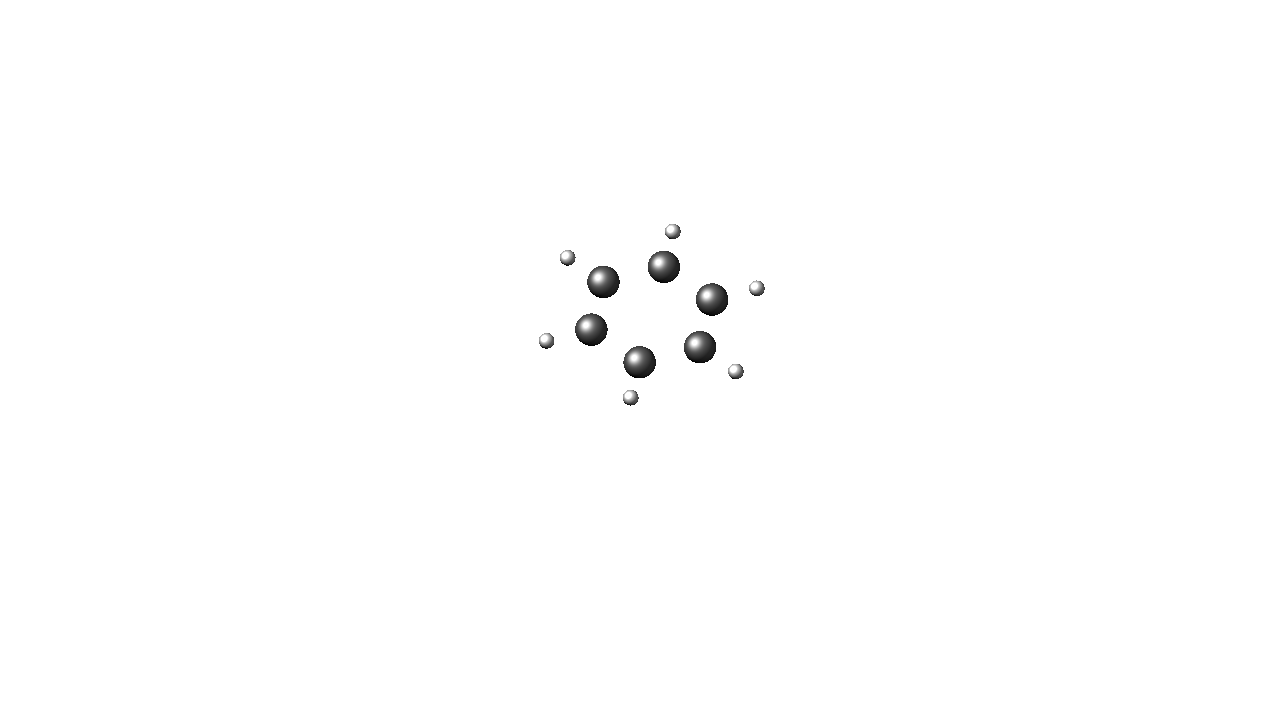
\includegraphics[width=0.40\textwidth]{c06h06}
    \bicaption{\quad 样图}{\quad Sample Figure}
    \label{fig:c06h06}
\end{figure}

如果插图的空白区域过大,以图片\verb|c06h06|为例,自动裁剪如图~\ref{fig:c06h06_trim}。
\begin{figure}[!htbp]
    \centering
    %trim option's parameter order: left bottom right top
    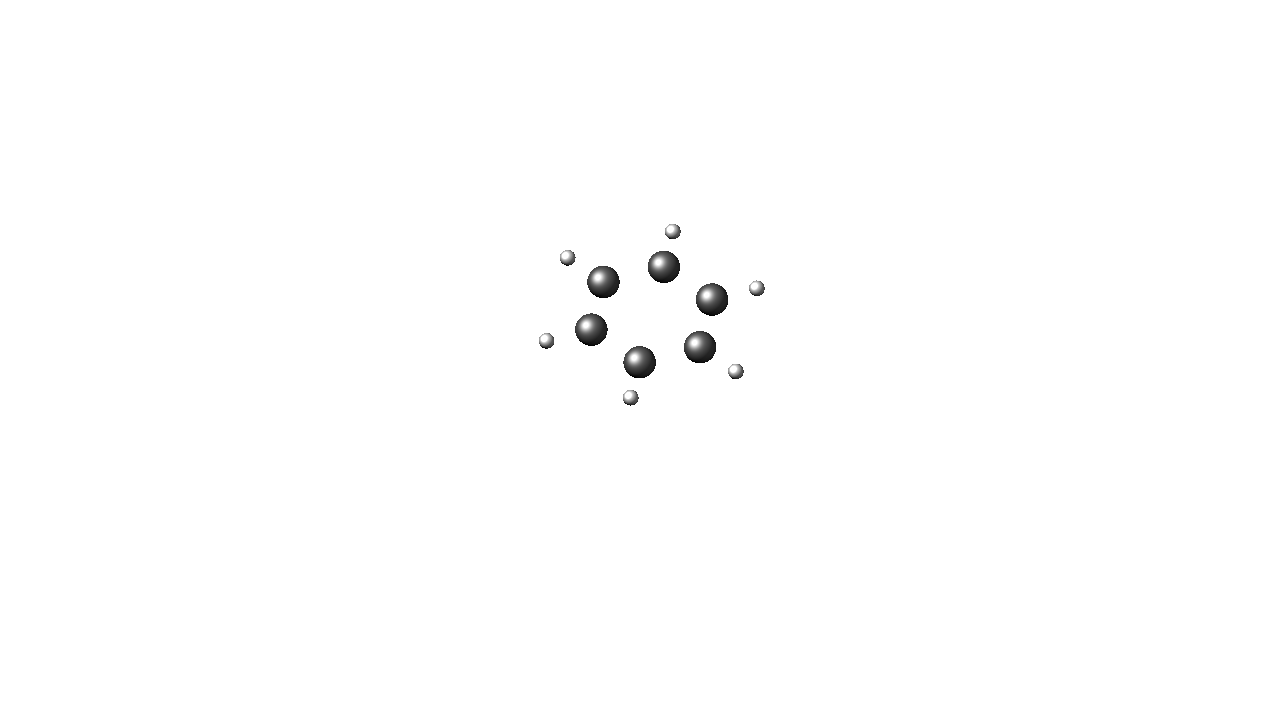
\includegraphics[trim = 60mm 80mm 60mm 60mm, clip, width=0.40\textwidth]{c06h06}
    \bicaption{\quad 自动裁切测试}{\quad Auto-Crop Test}
    \label{fig:c06h06_trim}
\end{figure}

多图的插入如图~\ref{fig:oaspl},多图不应在子图中给文本子标题,只要给序号,并在主标题中进行引用说明。
\begin{figure}[!htbp]
    \centering
    \begin{subfigure}[b]{0.35\textwidth}
      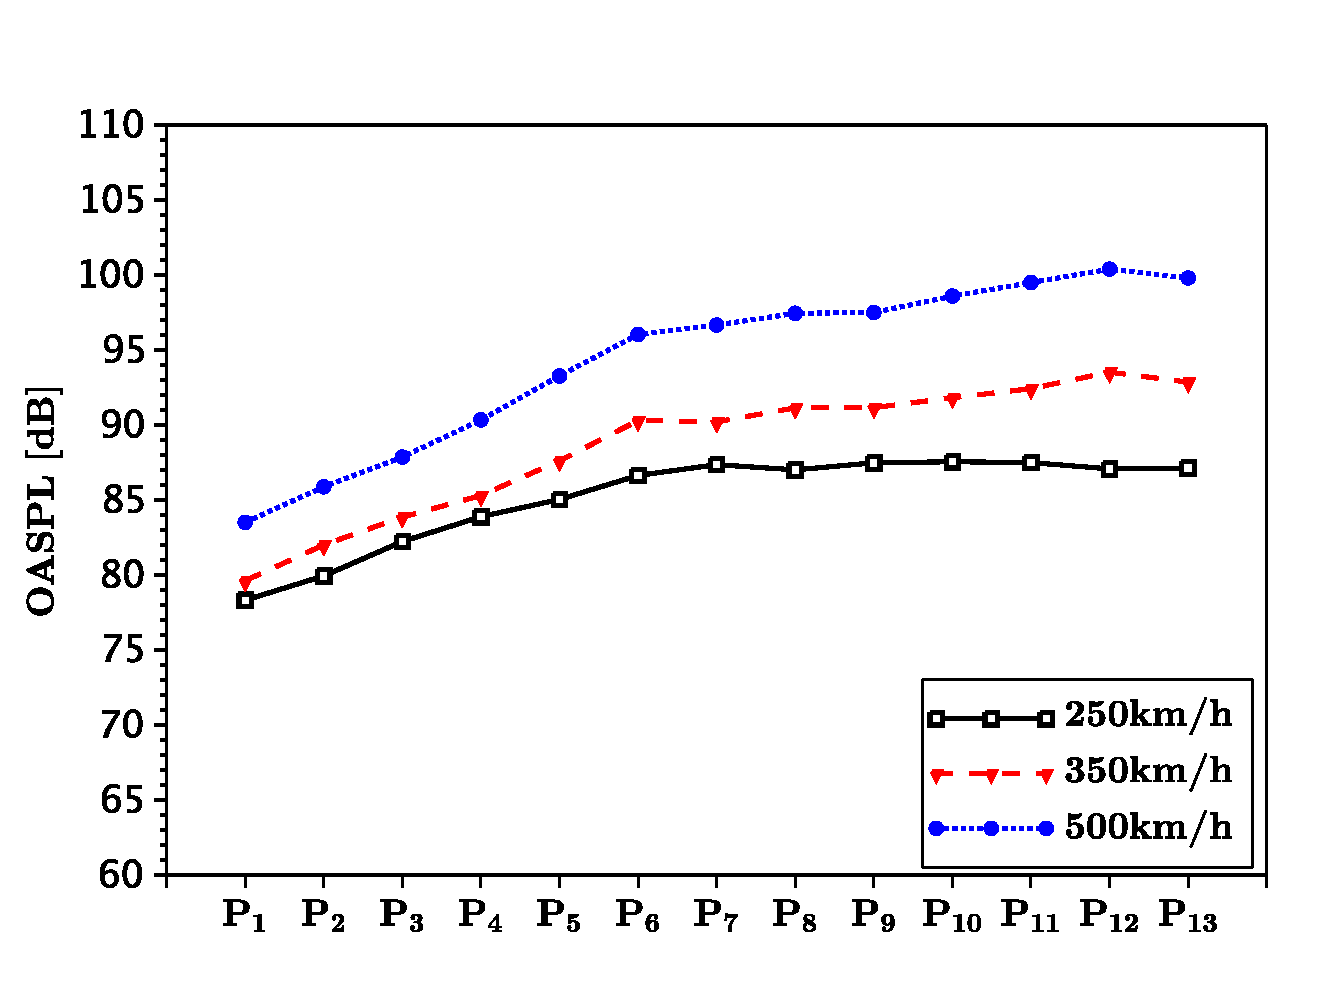
\includegraphics[width=\textwidth]{oaspl_a}
      \caption{}
      \label{fig:oaspl_a}
    \end{subfigure}%
    ~% add desired spacing
    \begin{subfigure}[b]{0.35\textwidth}
      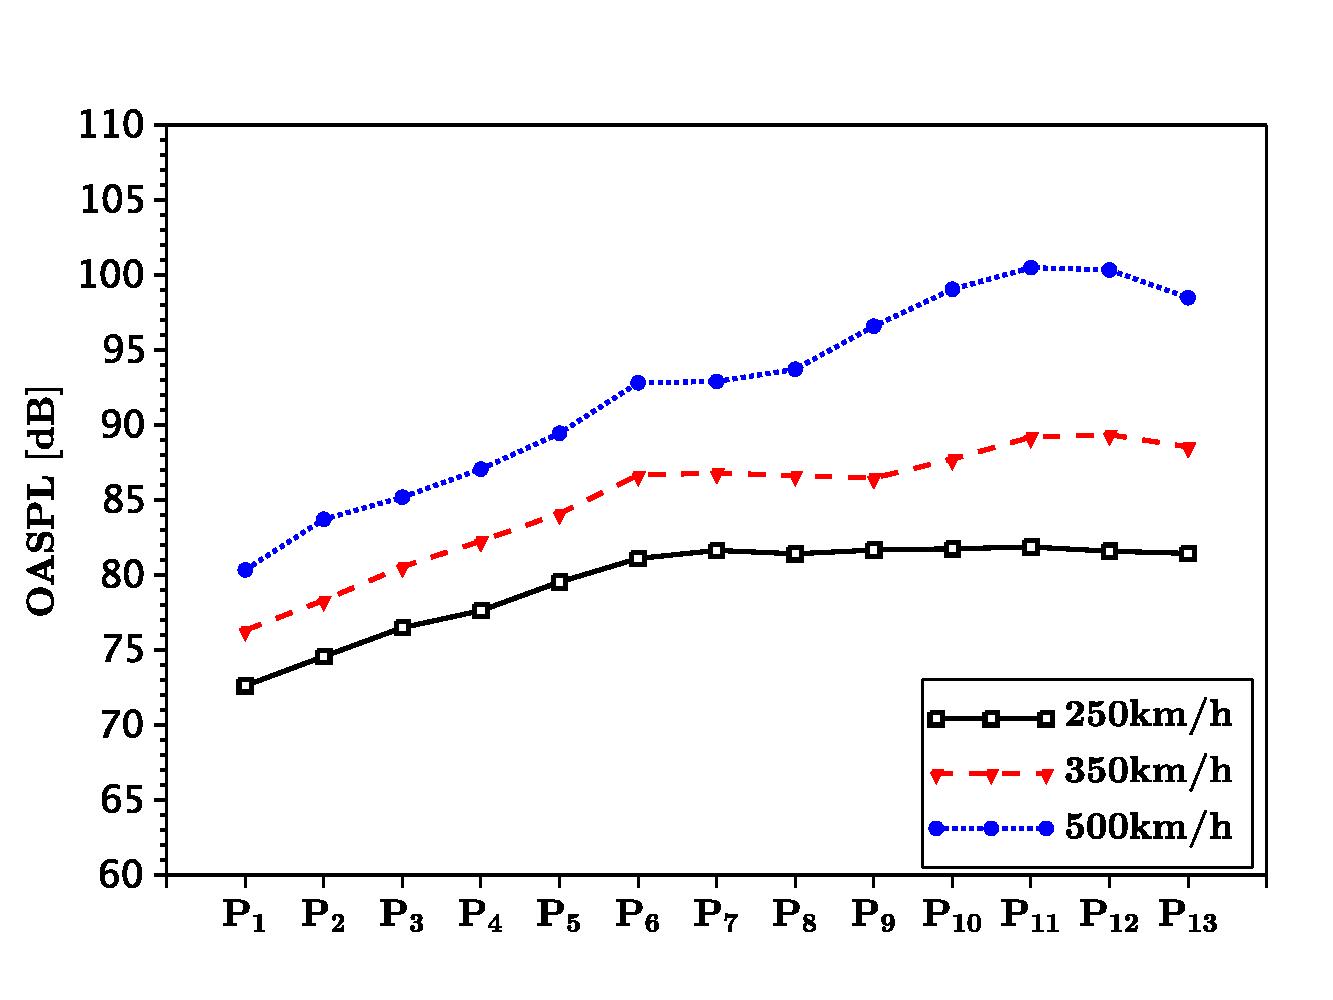
\includegraphics[width=\textwidth]{oaspl_b}
      \caption{}
      \label{fig:oaspl_b}
    \end{subfigure}
    \\% line break
    \begin{subfigure}[b]{0.35\textwidth}
      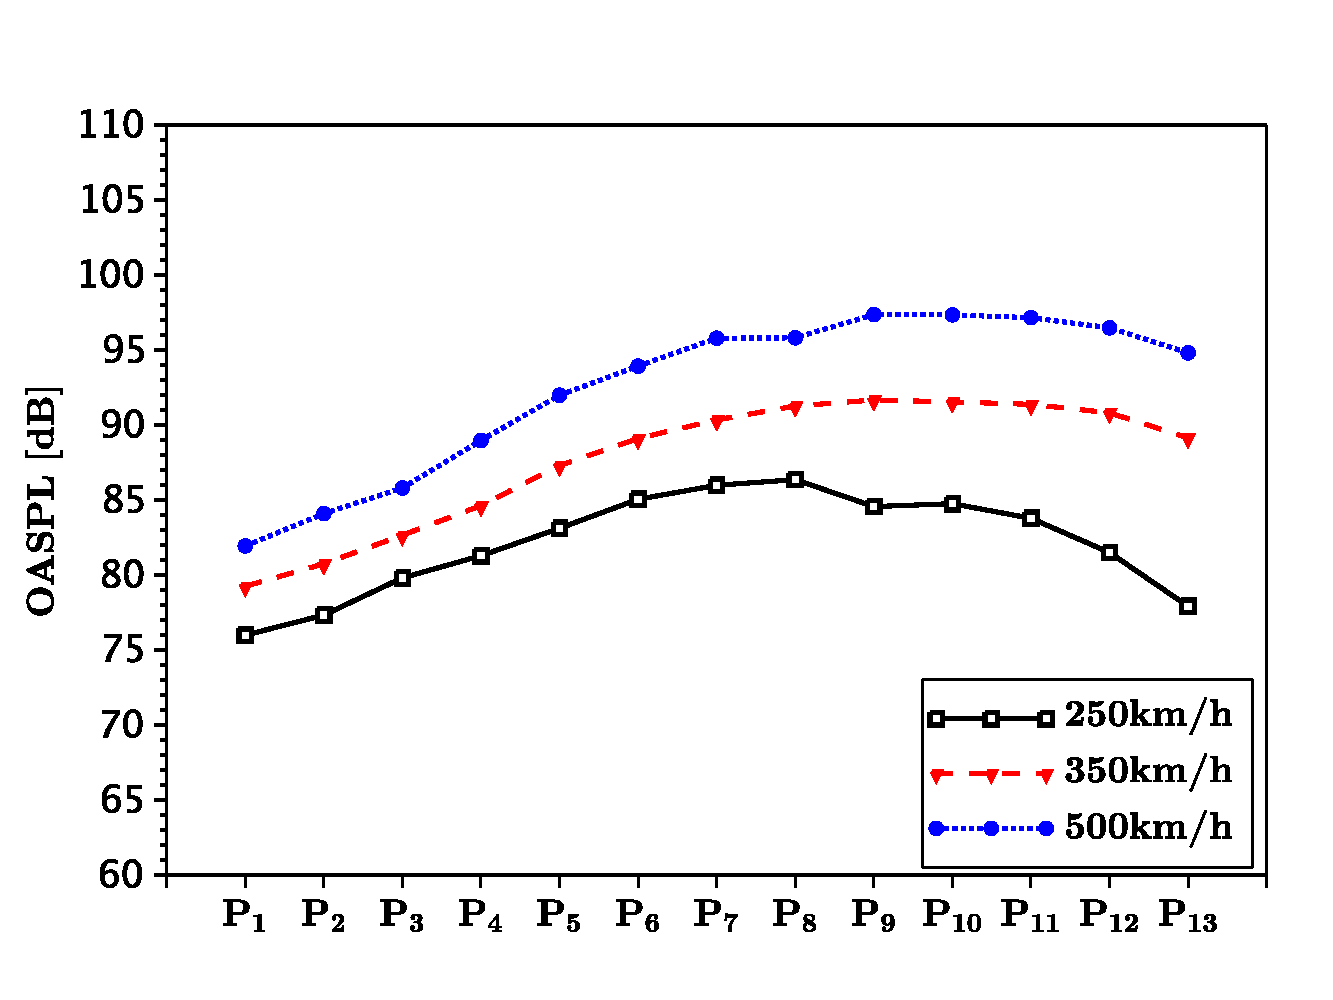
\includegraphics[width=\textwidth]{oaspl_c}
      \caption{}
      \label{fig:oaspl_c}
    \end{subfigure}%
    ~% add desired spacing
    \begin{subfigure}[b]{0.35\textwidth}
      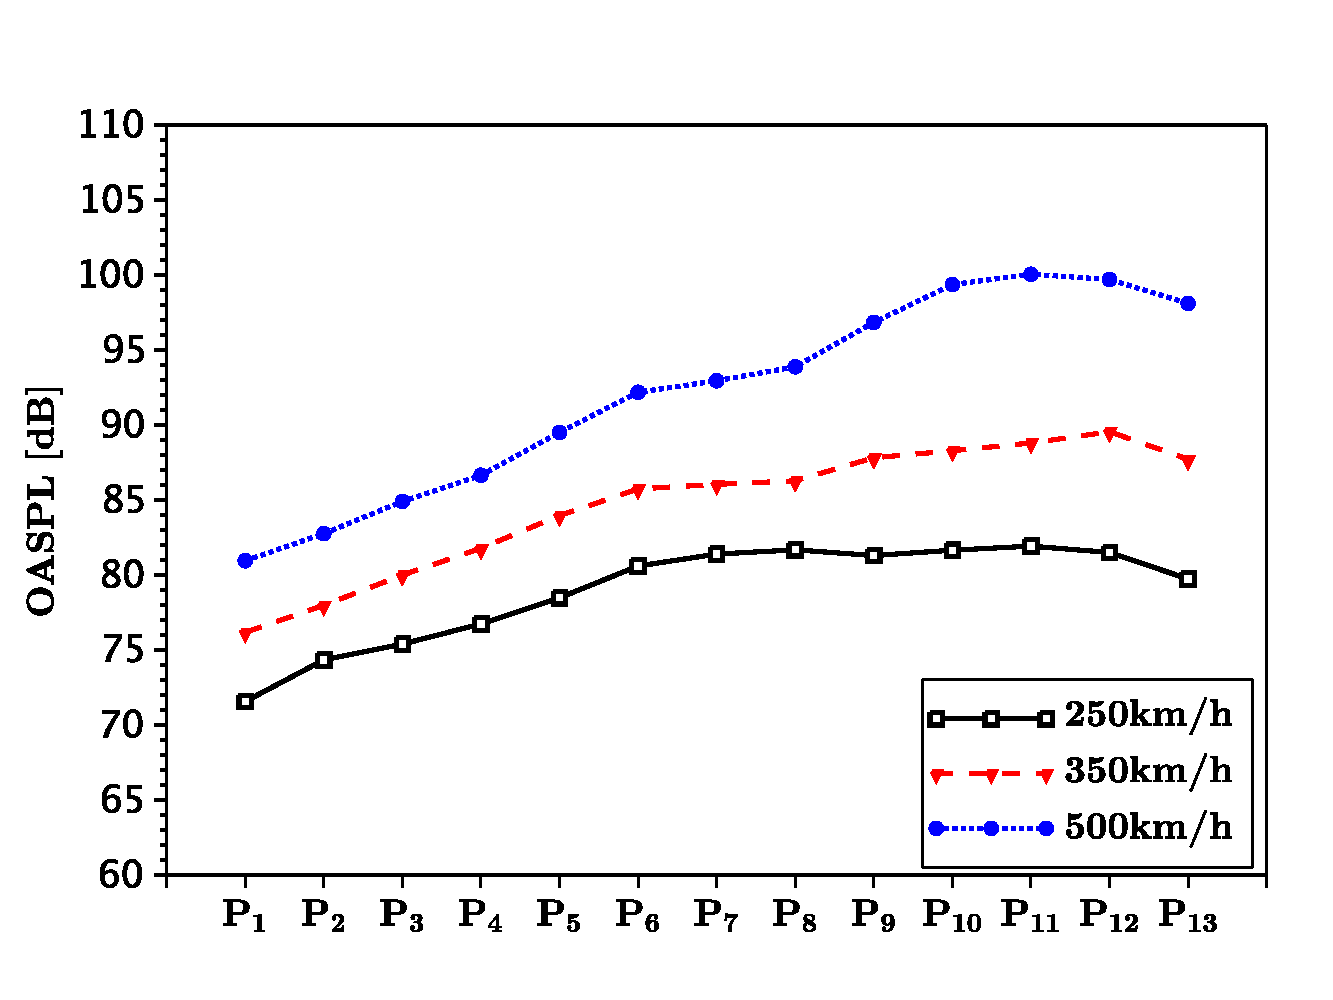
\includegraphics[width=\textwidth]{oaspl_d}
      \caption{}
      \label{fig:oaspl_d}
    \end{subfigure}
    \bicaption{\quad 多子图测试}{\quad A test for multi-subfig}
    \label{fig:oaspl}
\end{figure}

\subsection{表}

请见表~\ref{tab:sample}。
\begin{table}[!htbp]
    \bicaption{\quad 这是一个样表}{\quad This is a sample table}
    \label{tab:sample}
    \centering
    \footnotesize% fontsize
    \setlength{\tabcolsep}{4pt}% column separation
    \renewcommand{\arraystretch}{1.2}%row space 
    \begin{tabular}{lcccccccc}
        \hline
        行号 & \multicolumn{8}{c}{跨多列的标题}\\
        %\cline{2-9}% partial hline from column i to column j
        \hline
        Row 1 & $1$ & $2$ & $3$ & $4$ & $5$ & $6$ & $7$ & $8$\\
        Row 2 & $1$ & $2$ & $3$ & $4$ & $5$ & $6$ & $7$ & $8$\\
        Row 3 & $1$ & $2$ & $3$ & $4$ & $5$ & $6$ & $7$ & $8$\\
        Row 4 & $1$ & $2$ & $3$ & $4$ & $5$ & $6$ & $7$ & $8$\\
        \hline
    \end{tabular}
\end{table}

制图制表的更多范例,请见 \href{https://github.com/mohuangrui/ucasthesis/wiki}{ucasthesis 知识小站} 和 \href{https://en.wikibooks.org/wiki/LaTeX/Tables}{WiKibook Tables}。

\subsection{参考文献引用}

参考文献引用过程以实例进行介绍,假设需要引用名为"Document Preparation System"的文献,步骤如下:

1)将Bib格式的参考文献信息添加到ref.bib文件中(此文件位于Biblio文件夹下),如直接粘贴自网站,请注意修改其格式。

2)索引第一行 \verb|@article{lamport1986document,|中 \verb|lamport1986document| 即为此文献的label (中文文献也必须使用英文label,一般遵照:姓氏拼音+年份+标题第一字拼音的格式),想要在论文中索引此文献,\verb|\citep{lamport1986document}|。如此处所示 \citep{lamport1986document}。

多文献索引用英文逗号隔开, 如此处所示 \citep{lamport1986document, chu2004tushu, chen2005zhulu}。

更多例子如:

Walls等\citep{walls2013drought}根据Betts\citep{betts2005aging} 的研究,首次提出......理论。其中关于......的研究\citep{walls2013drought, betts2005aging},是当前中国得到迅速发展的研究领域 \citep{chen1980zhongguo, bravo1990comparative}。

不同文献样式和引用样式,如著者-出版年制(authoryear)、顺序编码制(numbers)、上标顺序编码制(super)可在Thesis.tex中对artratex.sty调用实现,详见 \href{https://github.com/mohuangrui/ucasthesis/wiki}{ucasthesis 知识小站之文献样式}。

%若在上标顺序编码制(super)模式下,希望在特定位置将上标改为嵌入式标,可使用 \citetns{niu2013zonghe,stamerjohanns2009mathml} 和 \citepns{niu2013zonghe,stamerjohanns2009mathml}。

参考文献索引的更多知识,请见 \href{https://en.wikibooks.org/wiki/LaTeX/Bibliography_Management}{WiKibook Bibliography}。\nocite{*}% 使文献列表显示所有参考文献(包括未引用文献)

\section{常见使用问题}\label{sec:qa}

设置文档样式: 在artratex.sty中搜索关键字定位相应命令,然后修改
\begin{enumerate}
    \item 正文行距:启用和设置 \verb|\linespread{1.25}|,默认1.25倍行距。
    \item 参考文献行距:修改 \verb|\setlength{\bibsep}{0.0ex}|
    \item 目录显示级数:修改 \verb|\setcounter{tocdepth}{2}|
    \item 文档超链接的颜色及其显示:修改 \verb|\hypersetup|
\end{enumerate}

文档内字体切换方法:
    \begin{itemize}
        \item 宋体:国科大论文模板ucasthesis 或 \textrm{国科大论文模板ucasthesis}
        \item 粗宋体:{\bfseries 国科大论文模板ucasthesis} 或 \textbf{国科大论文模板ucasthesis}
        \item 黑体:{\sffamily 国科大论文模板ucasthesis} 或 \textsf{国科大论文模板ucasthesis}
        \item 粗黑体:{\bfseries\sffamily 国科大论文模板ucasthesis} 或 \textsf{\bfseries 国科大论文模板ucasthesis}
        \item 仿宋:{\ttfamily 国科大论文模板ucasthesis} 或 \texttt{国科大论文模板ucasthesis}
        \item 粗仿宋:{\bfseries\ttfamily 国科大论文模板ucasthesis} 或 \texttt{\bfseries 国科大论文模板ucasthesis}
        \item 楷体:{\itshape 国科大论文模板ucasthesis} 或 \textit{国科大论文模板ucasthesis}
        \item 粗楷体:{\bfseries\itshape 国科大论文模板ucasthesis} 或 \textit{\bfseries 国科大论文模板ucasthesis}
    \end{itemize}

\let\cleardoublepage\relax
}

\chapter{中国科学院大学
研究生学位论文撰写规范指导意见(节选)}
{
\let\cleardoublepage\relax
}
学位论文是研究生在掌握已有的科学知识的基础上,运用科学思维和一定的科学方法、技术与工具,面向特定的科学领域所存在的科学问题,开展创新性研究而产生的科学研究成果。

学位论文是研究生科研工作成果的集中体现,是评判学位申请者学术水平、授予其学位的主要依据,是科研领域重要的文献资料。撰写学位论文是对研究生科学研究能力的基本训练,是研究生学业与研究成效的基本检验,也是科研与创新能力的重要体现。

为提高研究生学位论文的撰写质量,促进学位论文在内容和格式上的规范化,参照《学位论文编写规则》(GB/T 7713.1—2006)、《信息与文献 参考文献著录规则》(GB/T 7714—2015)和《学术出版规范 期刊学术不端行为界定》(CY/T 174—2019)等国家有关标准,特制定本指导意见(2021年修订)。各学科群学位评定分委员会(以下简称各学科群分会)可结合本学科领域的特点,参考本指导意见,制订符合本学科领域特点与要求的学位论文撰写具体要求。

本指导意见从2023年冬季批次开始实施。

\section{组成及要求}
学位论文一般由以下几个部分组成:封面、原创性声明及授权使用声明、摘要、目录、符号说明(若有)、正文、参考文献、附录(若有)、致谢、作者简历及攻读学位期间发表的学术论文与其他相关学术成果等。
\subsection{封面}
一律采用中国科学院大学规定的统一中英文封面,封面包含内容如下:

\begin{enumerate}
    \item 密级,涉密或延迟公开论文必须在论文封面标注密级,同时注明保密年限。公开论文不标注密级,可删除此行。
    \item 论文题目,应简明扼要地概括和反映整个论文的核心内容,一般不宜超过25个汉字(符),英文题目一般不应超过150个字母,必要时可加副标题。题目中应尽量避免使用缩略词、首字母缩写词、字符、代号和公式等。
    \item 作者姓名,根据《中国人名汉语拼音字母拼写规则》(GB/T 28039—2011),英文封面中的姓和名分写,姓在前,名在后,姓名之间用空格分开。姓和名需写全拼,姓全大写,名首字母大写。外国留学生姓名书写顺序以护照格式为准,字母全部大写。
    \item 指导教师,需同时填写导师姓名、专业技术职务和工作单位。如果有多位导师(均需经培养单位批准,并在学籍系统备案),第一导师在前,第二导师等依次在后。学位论文在指导小组的指导下完成的,应注明指导小组成员相应信息。
    \item 学位类别,包括学科门类(学术型)或专业学位类别以及学位级别。学科门类如理学、医学等,专业学位类别如应用统计、工商管理等。学位级别包括硕士、博士。
    \item 学科专业,填写攻读学位的一级学科/二级学科或专业学位类别/领域全称,须与学籍信息一致,不可用简写。
    \item 培养单位,填写就读研究所或学院、系全称,如中国科学院××研究所、中国科学院大学××学院。
    \item 时间,填写论文提交学位授予单位的年月,使用阿拉伯数字标注。一般夏季申请学位的论文标注6月,冬季申请学位的论文标注12月。例如:2023年6月,2023年12月。
\end{enumerate}

\subsection{原创性声明及授权使用声明}
本部分内容提供统一的模版,提交时作者和导师须亲笔签名。如遇导师无法签字时,培养单位应做出适当处理。
\subsection{摘要和关键词}
论文摘要包括中文摘要和英文摘要(Abstract)两部分。论文摘要应概括地反映出本论文的主要内容,说明本论文的主要研究目的、内容、方法、结论。要突出本论文的创造性成果或新见解,不宜使用公式、图表、表格或其他插图材料,不标注引用文献。中文摘要的字数由各学科群分会根据本分会涉及学科专业的特点提出具体要求。英文摘要与中文摘要内容应保持一致。留学生用其他语种撰写学位论文时,应有详细的中文摘要,字数由各学科群分会具体制定,建议一般不少于5000字。

摘要最后注明本文的关键词(3~5个)。关键词是为了文献标引和检索工作,从论文中选取出来,用以表示全文主题内容信息的单词或术语。关键词以显著的字符另起一行并隔行排列于摘要下方,左顶格,中文关键词间用中文逗号隔开。英文关键词应与中文关键词对应,首字母应大写,用英文逗号隔开。

摘要应另起一页,与正文前的内容连续编页(用罗马字符)。
\subsection{目录}
目录应包括论文正文中的全部内容的标题,以及参考文献、附录(若有)和致谢等,不包括中英文摘要。目录页由论文的章、条、附录等序号、名称和页码组成。正文章节题名要求最多编到第三级标题,即×.×.×(如1.1.1)。一级标题顶格书写,二级标题缩进一个汉字符位置,三级标题缩进两个汉字符位置。论文中若有图表,应有图表目录,置于目录页之后,另页编排。图表目录应有序号、图题或表题和页码。

目录应另起一页,与正文前的内容连续编页(用罗马字符)。
\subsection{符号说明(若有)}
如果论文中使用了大量的物理量符号、标志、缩略词、专门计量单位、自定义名词和术语等,应编写成注释说明汇集表。若上述符号等使用数量不多,可以不设此部分,但必须在论文中首次出现时加以说明。
论文中若有符号说明,应置于目录之后、正文之前,另起一页,与正文前的内容连续编页(用罗马字符)。
\subsection{正文}
正文一般包括绪论、论文主体、研究结论与展望等部分。

\begin{enumerate}
    \item 绪论应包括选题的背景和意义,国内外相关研究成果与进展述评,本论文所要解决的科学与技术问题、所运用的主要理论和方法、基本思路和论文结构等。绪论应独立成章,用足够的文字叙述,不与摘要雷同。要实事求是,不夸大也不弱化前人的工作和自己的工作。
    \item 论文主体是正文的核心部分,占主要篇幅,它是将学习和研究过程中调查、观察和测试所获得的材料和数据,经过思考判断、加工整理和分析研究,进而形成论点。依据学科专业及具体选题,论文主体可以有不同的表现形式,可以按照章与节的结构表述,也可以按照“研究背景与意义—研究方法与过程—研究结果与讨论”的表述形式组织论文。但主体内容必须实事求是,客观诚实,准确完备,合乎逻辑,层次分明,简明可读。
    \item 研究结论是对整个论文主要成果的总结,不是正文中各章小结的简单重复,应准确、完整、明确、精炼。应明确凝练出本研究的主要创新点,对论文的学术价值和应用价值等加以分析和评价,说明本项研究的局限性或研究中尚难解决的问题,并提出今后进一步在本研究方向进行研究工作的设想或建议。结论部分应严格区分本人研究成果与他人科研成果的界限。
\end{enumerate}
\subsection{参考文献}
本着严谨求实的科学态度撰写论文,凡学位论文中有引用或参考、借鉴他人思想或成果之处,均应按一定的引用规范,列于文末(通篇正文之后),参考文献部分应与正文的文献引用一一对应,注重合理引用,严禁抄袭剽窃等学术不端行为。
\subsection{附录(若有)}
主要列入正文内过分冗长的公式推导、供查读方便所需的辅助性数学工具或表格、数据图表、程序全文及说明、调查问卷、实验说明等。
\subsection{致谢}
对给予各类资助、指导和协助完成研究工作,以及提供各种对论文工作有利条件的单位及个人表示感谢。致谢应实事求是,切忌浮夸与庸俗之词。致谢末尾应具日期,日期与论文封面一致。
\subsection{作者简历及攻读学位期间发表的学术论文与其他相关学术成果}
作者简历应包括从大学起到申请学位时的个人学习工作经历。按学术论文发表的时间顺序,列出作者本人在攻读学位期间发表或已录用的学术论文清单(著录格式同参考文献)。其他相关学术成果可以是申请的专利、获得的奖项及完成的项目等代表本人学术成就的各类成果。


\section{撰写要求}

\subsection{学位论文基本要求}
学位论文必须是一篇系统的、完整的学术论文,遵循既定的学术规范与要求,不仅要符合学位论文的形式规范,更要符合学位论文的质量规范。做到:学术观点明确,立论正确,方法科学,材料翔实,数据可靠,推理严谨,论证充分,引用规范,结构合理,层次分明,文字通顺,表达准确,学风严谨。研究成果体现作者独到的学术见解、科学论证与创新性结论,表明作者掌握了坚实的基础理论和系统的专门知识,具有独立地从事科学研究的能力。

硕士学位论文选题应为本学科重要领域,有一定的理论意义或应用价值;在理论或方法上有一定的创新,解决了科学或生产实践中某一项重要的问题,取得重要的研究成果,具有较好的社会效益或应用前景。

博士学位论文选题应为本学科前沿领域,有重要的理论意义或应用价值;在理论或方法上有较大的创新,解决了科学或生产实践中某一项重大的问题,取得突破性的研究成果,具有重要的社会效益或应用前景。

\subsection{论文原创性要求}

学位论文应为学位申请者在导师的指导下独立完成的科学研究成果,为作者本人的原创性成果,系研究生经过多年的专业学习和科学研究,运用科学思维、科学方法或工具,探索科学领域中的某一科学问题,提出问题,分析问题,解决问题。学位论文中要有清晰完整的文献综述,但不能以文献综述来代替学位论文。论文引用规范合理,没有伪造、篡改、剽窃、他人代写、论文买卖及其它学术不端行为。

\subsection{论文创新性要求}

学位论文的研究既包括创造知识,即创新、发现和发明,是对未知世界及其规律的探索,也包括整理知识,即对已有知识分析整理,使其规范化、系统化,是对已有知识的传承。创新活动,贯穿了学位论文研究与写作的全过程,如提出新的学术思想、科学概念、假说、学说、定理、定律,设计新的观察方法和实验手段,建立新的科学模型,研制出新的产品,设计出新的工艺流程,发现新的物种等。学位论文的价值在于探索未知,发现科学发展中的规律与特征。学位论文要体现其应有的严谨性与探索性,在原创性的基础上实现对已有知识的超越、突破或颠覆,发现前所未有的科学问题,提出前所未有的分析论证,得出前所未有的科学结论。

\subsection{学位论文的字数要求}
学位论文最重要的意义在于其学术研究的创新性,应将学位论文的质量水平作为主要考量,不以字数多少作为特别要求,但各学科群分会可根据本领域涉及的学科专业特点做相应规定。

\subsection{文字、标点符号和数字}

除外国来华留学生、外语专业研究生以及特殊需要外,学位论文一律用国家正式公布实施的简化汉字书写。标点符号的用法以《标点符号用法》(GB/T 15834—2011)为准。数字用法以《出版物上数字用法》(GB/T 15835—2011)为准。

外国来华留学生可用中文或英文撰写学位论文,但应有详细的中英文摘要。外语专业的学位论文应用所学专业相应的语言撰写,摘要应使用中文和所学专业相应的语言对照撰写。

为了便于国际合作与交流,中文学位论文亦可有英文或其他文字的副本。

\subsection{论文正文}

\subsubsection{章节和各章标题}
论文正文须由另页右页(奇数页)开始,用阿拉伯数字连续编码,一直到全文最后。正文内部新章节无须另页右页(奇数页)开始。
    论文可参考“绪论-研究背景与意义-研究方法与过程-研究结果与讨论-研究结论与展望”的结构形式撰写,各主体研究内容可分别单独成为章节并作为章节标题使用。

各章标题中尽量不采用英文缩写词,对必须采用者,应使用本行业的通用缩写词。标题中尽量不使用标点符号。
\subsubsection{序号}
\textbf{标题序号}

论文标题分层设序。层次以少为宜,根据实际需要选择。各层次标题一律用阿拉伯数字连续编号。以三级标题为宜,最多四级。若确需要再增加一级,以小括号形式表示;不同层次的数字之间用小圆点“.”相隔,末位数字后面不加点号,如“1.1”,“1.1.1”等;章的标题居中排版,各层次的序号均左起顶格排,序号与题名间空一个汉字符。

\textbf{图表等编号}

论文中的图、表、附注、公式、算式等,一律用阿拉伯数字分章依序连续编码。其标注形式应便于互相区别,如:图1-1(第1章第一个图)、图2-2(第2章第二个图);表3-2(第3章第二个表)等。附录的图表参考正文的编号方式,如附图1-1或附表1-1。

\textbf{页码}

正文页码从绪论开始按阿拉伯数字(1,2,3……)连续编排,页码应位居左页左下角、右页右下角;正文前的部分(中英文摘要、目录等)用大写罗马数字(I,II,III…)单独编排,页码位于页面下方居中。
\subsubsection{页眉}
页眉从摘要开始,奇数页上标明“摘要”、“Abstract”、“目录”、“图表目录”等,偶数页上标明论文题目(英文摘要标明英文题目)。正文(即第1章开始到最后一章)的页眉,奇数页上标明每一章名称,偶数页上标明论文题目。参考文献、附录、致谢等的页眉,奇数页标明“参考文献”、“附录”、“致谢”等,偶数页标明论文题目。页眉居中设置。

\subsubsection{名词和术语}
科技名词术语及设备、元件的名称,应采用全国科学技术名词审定委员会公布的权威标准或其他相关权威信息源规定的术语或名称。标准中未规定的术语要采用行业通用术语或名称。全文名词术语必须统一。一些特殊名词或新名词应在适当位置加以说明或注解。双名法的生物学名部分均为拉丁文,并为斜体字。

采用英语缩写词时,除本行业广泛应用的通用缩写词外,文中第一次出现的缩写词应该用括号注明英文原词。新的外来名词应用括号注明英语全称和缩写语。

\subsubsection{量和单位}

量和单位要严格执行《国际单位制及其应用》(GB 3100-93)、《有关量、单位和符号的一般原则》(GB3101—93)有关量和单位的规定。量的符号一般为单个拉丁字母或希腊字母,并一律采用斜体(pH例外)。

\subsubsection{图和表}

论文中若有图和表,应设置图表目录,先列图后列表,置于目录页后,另页编排。

\textbf{(1) 图}

图片大小适当,图边界在页面范围内(图边界离页面边界距离大于页边距)。若图片中包含文字,文字大小不超过正文文字大小。
图包括曲线图、构造图、示意图、框图、流程图、记录图、地图、照片等,宜插入正文适当位置。引用的图必须注明来源。具体要求如下
\begin{itemize}
    \item 图应具有“自明性”,即只看图、图题和图注,不阅读正文,就可理解图意。每一图应有简短确切的图题,连同图序置于图下居中。
    \item 图中的符号标记、代码及实验条件等,可用最简练的文字横排于图框内或图框外的某一部位作为图注说明,全文统一。图题建议用中文及英文两种文字表达。
    \item 照片图要求主要显示部分的轮廓鲜明,便于制版,如用放大、缩小的复制品,必须清晰,反差适中,照片上应有表示目的物尺寸的标尺。
    \item 图片一般设为高6cm×宽8cm,但高、宽也可根据图片量及排版需要按比例缩放。中文(宋体)英文(Times New Roman)图注为五号字,1.25倍行距。
    \item 文中尽量不用世界地图、全国地图!如果一定要用,凡涉国界图件(国内部分地区、全国、世界部分地区、全球)必须使用自然资源部标准地图底图(下载网址:http://bzdt.ch.mnr.gov.cn),所用底图边界要完全无修改(包括南海诸岛位置),为适应排版时图的缩放,比例尺一律用线段比例尺,而不用数字比例尺。并在图题下注明“注:该图基于自然资源部标准地图服务网站下载的审图号为GS(2021)××××号的标准地图制作,底图边界无修改。”
\end{itemize}


\textbf{(2) 表}

表的编排一般是内容和测试项目由左至右横读,数据依序竖排,应有自明性,引用的表必须注明来源。具体要求如下:
\begin{itemize}
    \item 每一表应有简短确切的题名,连同表序置于表上居中。必要时,应将表中的符号、标记、代码及需说明的事项,以最简练的文字横排于表下作为表注。表题建议用中文及英文两种文字表达。
    \item 表内同一栏数字必须上下对齐。表内不应用“同上”、“同左”等类似词及“″”符号,一律填入具体数字或文字,表内“空白”代表无此项,“—”或“…”(因“—”可能与代表阴性反应相混)代表未发现,“0”该表实测结果为零。表内未测出值可以用“N.D. ”表示。
    \item 表格尽量用“三线表”,避免出现竖线,避免使用过大的表格,确有必要时可采用卧排表,正确方位应为“顶左底右”,即表顶朝左,表底朝右。表格太大需要转页时,需要在续表表头上方注明“续表”,表头也应重复排出。
    \item 中文(宋体)英文(Times New Roman)表注为五号字,1.25倍行距。
\end{itemize}

\subsubsection{表达式}
论文中的表达式需另行起,原则上应居中。若有两个以上的表达式,应从“1”开始的阿拉伯数字进行编号,并将编号置于括号内。编号采用右端对齐。表达式较多时可分章编号。

较长的表达式如必须转行,只能在+,-,×,÷,<,>等运算符之后转行,序号编于最后一行右顶格。

\subsection{参考文献}
参考文献格式规范参照《信息与文献 参考文献著录规则》(GB/T 7714—2015),或可参照国际刊物通行的参考文献格式。各学科群分会可根据本学科的一般规范制定相应的参考文献格式。文后参考文献和参考文献在正文中的标注方式可采用“顺序编码制”或“著者—出版年制”。确定采用某种方法后,文后参考文献和参考文献在正文中的标注方式要对应。

文后参考文献按“顺序编码制”组织时,各篇文献应按正文部分首次引用时标注的序号依次列出;文后参考文献按“著者—出版年制”组织时,条目不排序号,先按语种分类排列,语种顺序是:中文、日文、西文、俄文、其他文种;然后按著者字序和出版年排列。中文和日文按第一著者的姓氏笔画排序,中文也可按汉语拼音字母顺序排列,西文和俄文按第一著者姓氏字母顺序排列。当一个著者有多篇文献并为第一著者时,该著者单独署名的文献排在前面(并按出版年份的先后排列),接着排该著者与其他人合写的文献。
文后参考文献加标题“参考文献”,并列入全文目录。
凡正文里标注了参考文献的,其文献都必须列入文后参考文献。文后参考文献应集中著录于正文之后,不分章节著录。
正文中未被引用但被阅读或具有补充信息的文献可集中列入附录中,其标题为“荐读书目”。

详细内容请参考《中国科学院大学研究生学位论文撰写规范指导意见》。

\section{排版与印刷要求}

\subsection{纸张与页面要求}
\begin{table}[h]
    \centering
        \bicaption{\quad 排版和印刷要求}{\quad Typography and Printing Requirements}
    \begin{tabular}{lc}
        \hline
        %\multicolumn{num_of_cols_to_merge}{alignment}{contents} \\
        %\cline{i-j}% partial hline from column i to column j
        项目名称 & 要求\\
        \hline
        纸张&A4(210mm×297mm),幅面白色\\
        页面设置&上、下2.54cm,左、右3.17cm,页眉、页脚距页边界1.5cm\\
        封面&采用国科大统一格式\\
        页眉&宋体小五号居中,英文和阿拉伯数字用Times New Roman体\\
        页码&Times New Roman体小五号 \\

        \hline
    \end{tabular}

    \label{tab:printrequirements}
\end{table}

\subsection{印刷及装订要求}
论文封面使用中国科学院大学统一的封面格式。学位论文用A4标准纸(210 mm×297 mm)打印、印刷或复印,按顺序装订成册。自中文摘要起双面印刷,之前部分单面印刷。中文摘要、英文摘要、目录、论文正文、参考文献、附录、致谢、作者简历及攻读学位期间发表的学术论文与其他相关学术成果等,均须由另页右页(奇数页)开始。论文必须用线装或热胶装订,不使用钉子装订。封面用纸一般为150克花纹纸(需保证论文封面印刷质量,字迹清晰、不脱落),博士学位论文封面颜色为红色,硕士学位论文封面颜色为蓝色。

\subsection{书脊}
学位论文的书脊用黑体,英文和阿拉伯数字用Times New Roman体,字号一般为小四号,可根据论文厚度适当调整。上方写论文题目,中间写作者姓名,下方写“中国科学院大学”,距上下边界均为3cm左右。
%---------------------------------------------------------------------------%
% main content
%-
%-> Appendix
%-

%-
%-> Backmatter: bibliography, glossary, index
%-
\backmatter% initialize the environment
\intotoc*{\cleardoublepage}{\bibname}% add link to toc
\artxifstreq{\artxbib}{bibtex}{% enable bibtex
    \bibliography{Biblio/ref}% bibliography
}{%
    \printbibliography% bibliography
}
\cleardoublepage%
\appendix% initialize the environment

\chapter{附录\quad 公式测试}

\begin{equation} \label{eq:appedns}
    \adddotsbeforeeqnnum%
    \begin{cases}
        \frac{\partial \rho}{\partial t} + \nabla\cdot(\rho\Vector{V}) = 0\\
        \frac{\partial (\rho\Vector{V})}{\partial t} + \nabla\cdot(\rho\Vector{V}\Vector{V}) = \nabla\cdot\Tensor{\sigma}\\
        \frac{\partial (\rho E)}{\partial t} + \nabla\cdot(\rho E\Vector{V}) = \nabla\cdot(k\nabla T) + \nabla\cdot(\Tensor{\sigma}\cdot\Vector{V})
    \end{cases}
    \nonumber
\end{equation}
\begin{equation}
    \adddotsbeforeeqnnum%
    \frac{\partial }{\partial t}\int\limits_{\Omega} u \, \mathrm{d}\Omega + \int\limits_{S} \unitVector{n}\cdot(u\Vector{V}) \, \mathrm{d}S = \dot{\phi}
    \nonumber
\end{equation}
\[
    \begin{split}
        \mathcal{L} \{f\}(s) &= \int _{0^{-}}^{\infty} f(t) e^{-st} \, \mathrm{d}t, \ 
        \mathscr{L} \{f\}(s) = \int _{0^{-}}^{\infty} f(t) e^{-st} \, \mathrm{d}t\\
        \mathcal{F} {\bigl (} f(x+x_{0}) {\bigr )} &= \mathcal{F} {\bigl (} f(x) {\bigr )} e^{2\pi i\xi x_{0}}, \ 
        \mathscr{F} {\bigl (} f(x+x_{0}) {\bigr )} = \mathscr{F} {\bigl (} f(x) {\bigr )} e^{2\pi i\xi x_{0}}
    \end{split}
\]

mathtext: $A,F,L,2,3,5,\sigma$, mathnormal: $A,F,L,2,3,5,\sigma$, mathrm: $\mathrm{A,F,L,2,3,5,\sigma}$.

mathbf: $\mathbf{A,F,L,2,3,5,\sigma}$, mathit: $\mathit{A,F,L,2,3,5,\sigma}$, mathsf: $\mathsf{A,F,L,2,3,5,\sigma}$.

mathtt: $\mathtt{A,F,L,2,3,5,\sigma}$, mathfrak: $\mathfrak{A,F,L,2,3,5,\sigma}$, mathbb: $\mathbb{A,F,L,2,3,5,\sigma}$.

mathcal: $\mathcal{A,F,L,2,3,5,\sigma}$, mathscr: $\mathscr{A,F,L,2,3,5,\sigma}$, boldsymbol: $\boldsymbol{A,F,L,2,3,5,\sigma}$.

vector: $\Vector{\sigma, T, a, F, n}$, unitvector: $\unitVector{\sigma, T, a, F, n}$

matrix: $\Matrix{\sigma, T, a, F, n}$, unitmatrix: $\unitMatrix{\sigma, T, a, F, n}$

tensor: $\Tensor{\sigma, T, a, F, n}$, unittensor: $\unitTensor{\sigma, T, a, F, n}$ 


% appendix content
\fancypagestyle{appendixheader}{
  \fancyhf{}
  \fancyhead[C]{\footnotesize 附录}%此处填写中文标题
  \fancyfoot[C]{\footnotesize \thepage}% page number
    \renewcommand{\headrulewidth}{0.8pt}% header rule
    \renewcommand{\footrulewidth}{0pt}% footer rule
}
\thispagestyle{appendixheader}

\backmatter% initialize the environment
%---------------------------------------------------------------------------%
%->> Backmatter
%---------------------------------------------------------------------------%
\chapter[致谢]{致\quad 谢}\chaptermark{致\quad 谢}% syntax: \chapter[目录]{标题}\chaptermark{页眉}
%\thispagestyle{noheaderstyle}% 如果需要移除当前页的页眉
%\pagestyle{noheaderstyle}% 如果需要移除整章的页眉

此处填写致谢。


\rightline{2023年6月}
\chapter{作者简历及攻读学位期间发表的学术论文与其他相关学术成果}

\section*{作者简历:}
××××年××月——××××年××月,在××大学××院(系)获得学士学位。

××××年××月——××××年××月,在××大学××院(系)获得硕士学位。

××××年××月——××××年××月,在中国科学院××研究所(或中国科学院大学××院系)攻读博士/硕士学位。

工作经历:

\section*{已发表(或正式接受)的学术论文:}

{
\setlist[enumerate]{}% restore default behavior
\begin{enumerate}[nosep]
    \item 已发表的工作1
    \item 已发表的工作2
\end{enumerate}
}

\section*{申请或已获得的专利:}

(无专利时此项不必列出)

\section*{参加的研究项目及获奖情况:}


\cleardoublepage[plain]% 让文档总是结束于偶数页,可根据需要设定页眉页脚样式,如 [noheaderstyle]
%---------------------------------------------------------------------------%
% other information
\end{document}
%---------------------------------------------------------------------------%

